\begin{figure}[H]
\centering
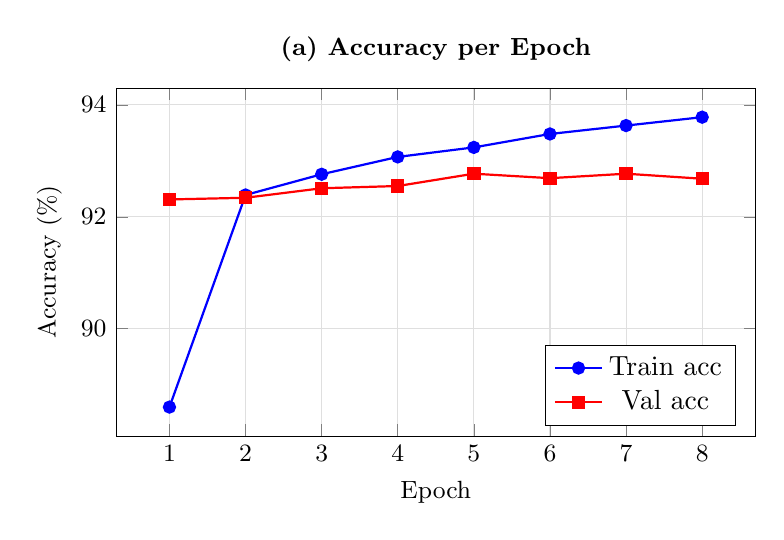
\begin{tikzpicture}
\begin{axis}[width=0.8\linewidth, height=6cm,
    title={\textbf{(a) Accuracy per Epoch}}, title style={font=\small\bfseries},
    xlabel={Epoch}, ylabel={Accuracy (\%)}, legend pos=south east,
    grid=both, grid style={gray!25}, tick label style={font=\small},
    label style={font=\small}]
\addplot[blue, mark=*, thick] coordinates {(1,88.6) (2,92.39) (3,92.76) (4,93.07) (5,93.24) (6,93.48) (7,93.63) (8,93.78)};
\addlegendentry{Train acc}
\addplot[red, mark=square*, thick] coordinates {(1,92.31) (2,92.34) (3,92.51) (4,92.55) (5,92.77) (6,92.69) (7,92.77) (8,92.68)};
\addlegendentry{Val acc}
\end{axis}\end{tikzpicture}

\vspace{0.6em}
\begin{tikzpicture}
\begin{axis}[width=0.8\linewidth, height=6cm,
    title={\textbf{(b) Loss and Validation Macro-F1}}, title style={font=\small\bfseries},
    xlabel={Epoch}, ylabel={Value}, legend pos=east,
    grid=both, grid style={gray!25}, tick label style={font=\small},
    label style={font=\small}]
\addplot[blue, mark=*, thick] coordinates {(1,0.3581198399991802) (2,0.2387861544474294) (3,0.2231587276087751) (4,0.2135670221261801) (5,0.2024068814309818) (6,0.1949770145315405) (7,0.1859950276236166) (8,0.1780524332567774)};
\addlegendentry{Train loss}
\addplot[red, mark=square*, thick] coordinates {(1,0.2616129814416212) (2,0.2355310806378111) (3,0.2495689039430585) (4,0.2255397201427041) (5,0.2524127918535373) (6,0.2644012832343568) (7,0.2789653191831522) (8,0.2722118142907294)};
\addlegendentry{Val loss}
\addplot[green!55!black, mark=triangle*, thick] coordinates {(1,0.8783128434314978) (2,0.8834907179543187) (3,0.8843035330987611) (4,0.8837239608350981) (5,0.8886306803690934) (6,0.8883763249047254) (7,0.8884991968524516) (8,0.8883047350251011)};
\addlegendentry{Val Macro-F1}
\end{axis}\end{tikzpicture}
\caption[Stage 2 training curves]{Stage~2 question-router training dynamics over
8 epochs. The best checkpoint (epoch~5) reaches 92.77\% validation accuracy and
0.8886 macro-F1.}
\label{fig:stage2_curves}
\end{figure}
